 \documentclass[12pt]{report}
\usepackage[utf8]{inputenc}
\usepackage[UKenglish]{babel}
\usepackage[margin=1in]{geometry}
\usepackage{amsmath}
\usepackage{graphicx}
\usepackage{mymacros}
\usepackage{setspace}
\onehalfspacing
% for changing font colour
\usepackage[dvipsnames]{xcolor}

\definecolor{darkRed}{RGB}{189, 20, 17} 
\definecolor{darkBlue}{RGB}{3, 45, 171}
\newcommand{\tcr}[1]{\textcolor{darkRed}{#1}}
\newcommand{\tcb}[1]{\textcolor{darkBlue}{#1}}


\title{4th Year Project - Final Report}
\author{jh2044}
\date{February 2020}

\begin{document}

\maketitle

\begin{abstract}
    This project aims to survey and analyse Concrete Canvas' new cement \tcr{impregnated cloth} production line in order to identify and characterise the mechanisms responsible for producing faulty material, as well as develop a \underline{specification} for an on-line computer vision based system capable of \underline{accurately} \tcr{identifying} these faults in real-time.
    
    \tcr{need a short paragraph on cement impregnated fabrics}
    
    The new product, CCX, is a \tcr{extruded} plastic  coated two layer stitch-bonded non-woven geo-textile with a cement-sand dry powder \tcr{infill}. \tcr{The/a} critical manufacturing step is a pressurised \tcr{dry} powder injection  through \tcr{280} parallel \tcr{5mm ID} aluminium tubes. This process is highly volatile and tube blockages occur creating regions of critically underfilled material. Additional failure mechanisms within the other manufacturing steps have been identified \tcr{including stitch drops etc}.
    
    \tcr{During the Summer 2019}, a qualitative analysis of the cement injection process was carried out; a number of phenomena were identified as potential indicators of the powder flow state in the tubes. The feasibility of measuring each of these phenomena was compared. A surface profile measurement using a laser profilometer was selected for further development due to its \tcr{WHYYYY}.
    
    An analysis of the manufacturing process was carried out in order to understand the parameters involved in producing the surface profile of the material. Additional failure mechanisms were identified at each step, and the \tcr{effect on the profile} was considered. \tcr{I feel there is more to be said here, maybe about how the analysis took place etc}.
    
    A profilometer test rig was designed \tcr{and built} \tcr{using a cylindrical datum surface with a tangential laser line, maybe more on this} in order to investigate the nature of the material surface profile in a \tcr{range} of samples. A measurement calibration system was developed. \tcr{maybe something about extending this rig to the production line}.
    
    \tcr{Section on experimentation: what was the experimental protocol, what were the aims, what data, results, discussion}
    
    \tcr{Section on future work}
    
    \tcr{Section on conclusions: What did we find out?, how do we know this?}
    
    
\end{abstract}

\tableofcontents

\pagebreak
\chapter{Introduction}
    
    Concrete Canvas is a cement impregnated geo-textile manufacturer. They currently have two products on the market: Concrete Canvas and CC-Hydro, both of which contain an internal spacer fabric that provides a containment void for the cement. The spacer is costly due to its complicated manufacturing process. In order to enter the low cost geo-textiles market, Concrete Canvas are developing a new alternative product, CCX. CCX does not include the internal spacer in its structure and only uses standard, low-cost components.
    
    CCX is in a late stage of development, with the final production line currently being designed, constructed and tested. \tcr{The development approach for CCX is agile, with continuous iteration of the design and operating parameters based on test results, rather than through extensive theoretical investigation. This technique allows for changes to be made at any stage during development, in order to improve the manufacturing process (better material quality/less wastage/faster production/basically more money in)}. \tcr{This development technique benefits from high quality and well-ordered test results that well represent the operation of the production line and thus how to optimise it. Currently, the testing data is in the form of unstructured qualitative observations, and some limited sample measurements are also taken (such as thickness observations, bending and tensile tests.}. 
    
    \section{Project Motivation}
        \tcb{What really motivates this project is  \textbf{defect detection and characterisation!! this is not really clearly stated below, as I'm being vague and wish washy still}}
        
        The existing production line contains a number of fabrication processes that \tcr{do not always work as intended (can change in an uncontrolled manner.} As such, the material produced is often obviously faulty. Additionally, a \tcr{quantitative specification} that describes the material in terms of its physical characteristics \tcr{(and the ranges/different possible values therein)} has not yet been produced.
        
        \tcr{Improving the understanding (be it through more data gathering, or a clearer picture of what is going on in the inner workings) of the critical operations of the production line (inputs/outputs/operations/parameters/known problems/potential problems) as a whole and of the material that is produced will enhance the ability to analyse the current state of operation of the production line. It will also facilitate the characterisation and diagnosis of any issues that arise. This will improve both the development of the production line, but also the normal operation as well. (in that it will give engineers/operators/technicians a baseline for logging/classifying/repairing/mitigating problems)}.

    \section{Literature Review}
    CV Defect Detection,
    \section{Aims and Objectives}
    
    \begin{itemize}
        \item \tcr{to translate production line parameter measurements from the temporal domain to the spacial domain}
        \item \tcr{Understand and structure the processes that are involved in making CCX, what goes in/comes out, what changes, what variables are associated, what can go wrong. How critical these things are in the end. Primarily identify the mechanisms that produce defects in the material}
        \item \tcr{Investigate on-line techniques to measure various aspects of the production line}
        \item \tcr{Investigate ways to characterise the material that comes out, in terms of how good it is basically}
        \item \tcr{develop a real-time warning system for serious material faults}
    \end{itemize}
        
\pagebreak
\chapter{Background}

    \tcr{need a short paragraph on cement impregnated fabrics}
    
    The new product, CCX, is a \tcr{extruded} plastic  coated two layer stitch-bonded non-woven geotextile with a cement-sand dry powder \tcr{infill}. \tcr{The/a} critical manufacturing step is a pressurised \tcr{dry} powder injection  through \tcr{280} parallel \tcr{5mm ID} aluminium tubes. This process is highly volatile and tube blockages occur creating regions of critically under-filled material. Additional failure mechanisms within the other manufacturing steps have been identified \tcr{including stitch drops etc}.
    
    \tcb{who is concrete canvas? where are they based?}
    \tcb{what is a geo-textile? What materials does this include?}
    
    
    \section{Concrete-Fabric Composites}
    \tcr{Geo-textile materials have a wide range of applications: ditch lining, bund lining, erosion protection, the list goes on}
    Concrete Canvas and CC-Hydro \tcb{why two, what are the differences, similarities?}
    
    \section{CCX Overview}
        \subsection{Material}
            need to descrube what the material is, what it is made up of, it's known properties, it's projected property targets. Individual component properties, manufacturing etc.
            Non-woven surface
            \addfigured{0.8}{example-image-c}{early manual surface measurements (where is that spreadsheet I wonder...}{surface_variation}
            \addfigured{.5}{1x_HH_surface.jpg}{HH (upper?) non-woven surface}{hh_1x}
            \addfigured{.5}{1x_HI_surface.jpg}{HH (lower?) non-woven surface}{hi_1x}
            \addfigured{.5}{5x_HH_calen.jpg}{HH (upper?) non-woven surface 5x microscopic view}{hh_5x}
            \addfigured{.5}{5x_HI_calen.jpg}{HI (lower?) non-woven surface 5x microscopic view}{hi_5x}
        \subsection{Production Line}
            overview
            
            this section will provide the background information as to what technology and systems are in place to make the material. mechanical process descriptions etc. 
            \addfigured{1}{process_flow_overview.pdf}{production line process flow overview}{ccx_process_overview}
            \addfigured{1}{CX02_V03_side_drawing.png}{production line physical overview}{ccx_line_overview}
            unwind stations 
            \addfigured{0.8}{example-image-a}{image of yarn unwind creole}{yarn_creole}
            \addfigured{0.8}{example-image-b}{image of unwind stand}{nw_unwind_stand}
            \addfigured{0.8}{example-image-c}{image of unwind stitching stand}{nw_inline_stitching}
            \addfigured{0.8}{example-image-a}{diagram to describe Maliwatt Stitchithing}{matliwatt_stitch}
            \addfigured{0.8}{example-image-b}{image to describe lances and injection}{cement_injection}
            \addfigured{0.8}{example-image-c}{image to describe extraction box}{extraction_box}
            something about accumulation here
            
            something about machine parameters, on a large scale (lengths, widths, speeds. But at the scale of the whole line. Individual parameters are included in the full analysis.
            \addfigured{0.8}{example-image-c}{table of machine parameters}{machine_parameters}
            
\chapter{Production Line Analysis}
    \section{Component Conveyance Model}
        
        \subsection{Continuous Web}
            
        \subsection{Yarn}
        \subsection{Powder and Plastic}
    \section{Process Analysis}
        \subsection{}
    \section{Material Defect Investigation}
\chapter{Material Surface Characterisation}
    \tcr{all notation is a work in progress and definitely subject to change and hopefully my explanation will solidify as I actually work out what I'm doing}
    \section{Raw Laser Line Image Processing}
        \begin{figure}[ht!]
            \centering
            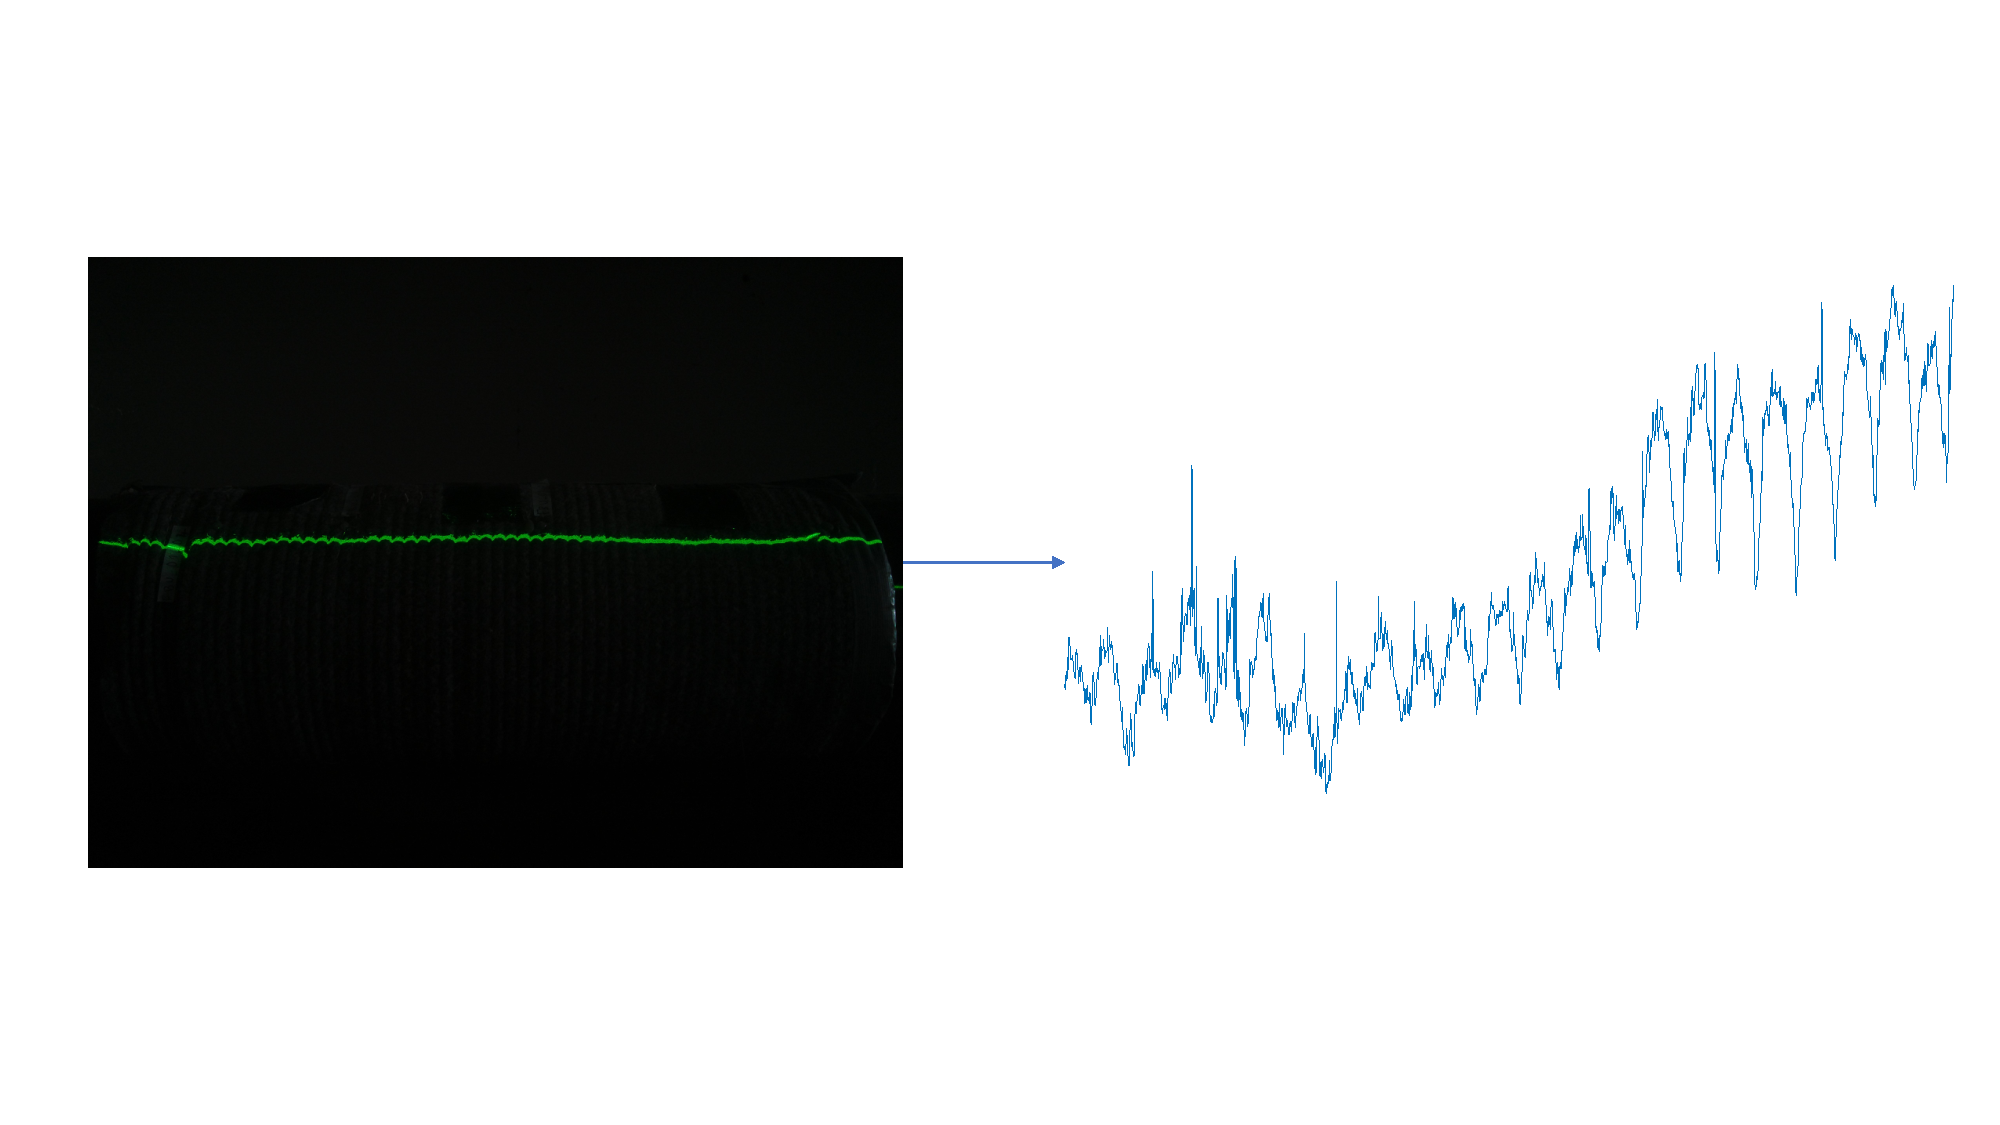
\includegraphics[width=\textwidth,trim={0 5cm 0 5cm},clip]{temp_height_measure.pdf}
            \caption{Raw Laser Line Image Processing}
        \end{figure}
        This process transforms each image into a calibrated estimate of the material surface. In summary:
        
        \begin{itemize}
            \item Crop image to relevant region
            \item Threshold image for laser light
            \item Compute estimate for the laser height at each pixel column by comparing the light intensities
            \item Transform camera coordinates into world coordinates.
            ie $(\text{column}, \text{row}) \rightarrow (x',z')$. This requires taking into account the laser plane to camera geometry, and a simple grid calibration in the plane of the laser can be used to generate static calibration constants.
            \item transform world coordinates into material coordinates: $(x',z') \rightarrow (x,y,z)$. This requires consideration of the laser plane to material surface geometry and a correspondence between the image acquisition time and the roller movement speed/position. \tcr{Note, we will likely average over the displacement of each measurement in the longitudinal ($y$) direction for simplicity}
        \end{itemize}
    
    \section{Profile Parameterisation}
        \begin{figure}
            \centering
            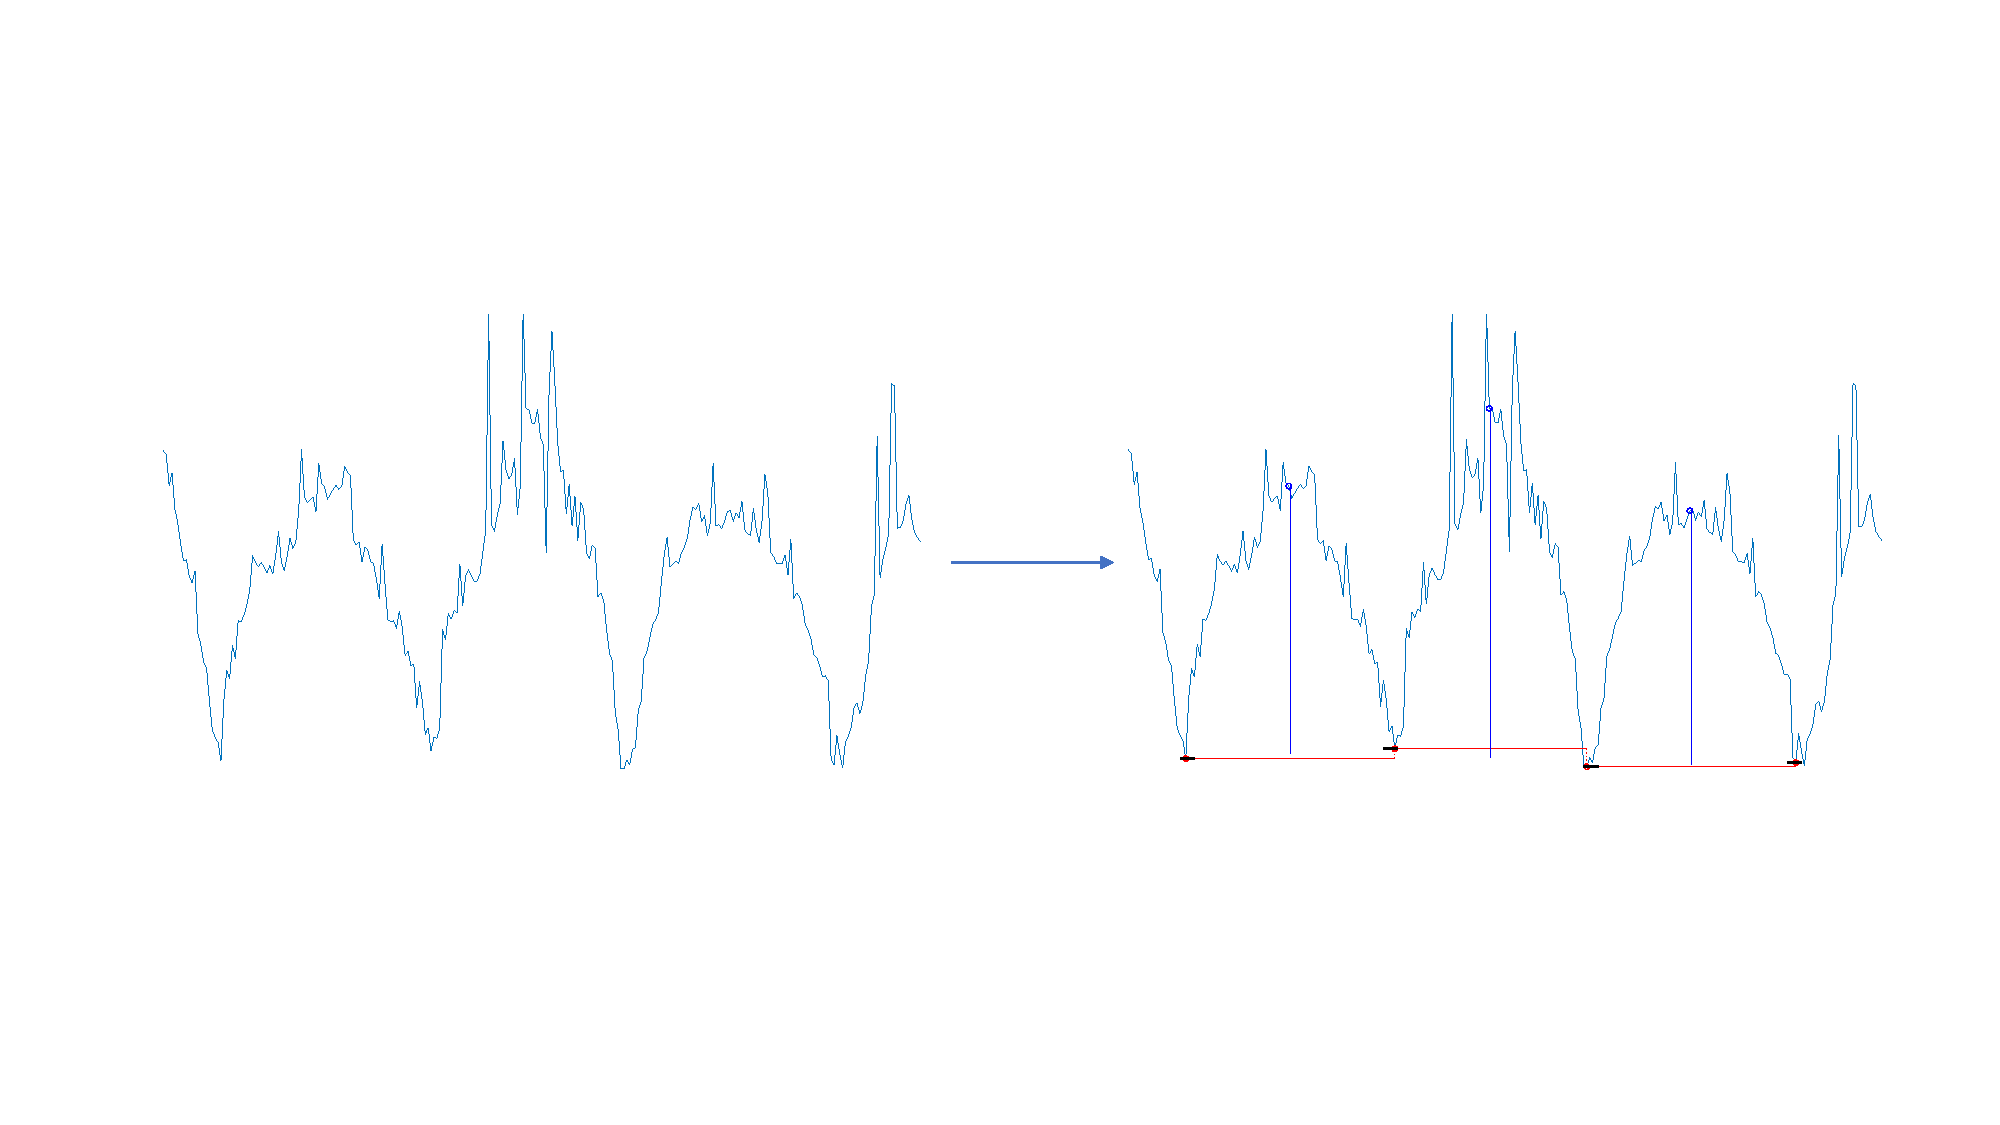
\includegraphics[width=\textwidth,trim={0 5cm 0 5cm},clip]{temp_parameterise.pdf}
            \caption{Profile Parameterisation}
        \end{figure}
        This process transforms each set of surface measurement points into a set of parameters corresponding to the bumps/stitch tracks on the surface.
        
        \begin{itemize}
            \item Compute stitch track locations 
            \item compute observed bump parameters $\pmb{\theta}^*_{ij}$
        \end{itemize}
        
        note that $\pmb{\theta}_{ij}$ corresponds to the $i$-th bump along the surface, at the $j$-th location in the longitudinal direction. also $\pmb{\theta} = [\theta_1,\theta_2,\ldots ,\theta_n]^T$ as some vector of parameters.
        
        The parameters describe elements of the bumps such as:
        \begin{itemize}
            \item width (trough-trough $x$ distance)
            \item relative height (trough-peak) height
            \item absolute height ($z$ position of troughs/peaks)
            \item curvature
            \item trough height change (trough-trough $z$ distance)
            \item surface fluffiness
        \end{itemize}
         
        This significantly reduces the size of the data-set by drawing out useful features of the profile that give an indication of the state of the observed profile in terms of its material characteristics. A careful choice of parameters is required in order to give an optimal trade-off between computational complexity and accuracy. If the parameterisation is too simplistic, it may cause not convey the required information about the surface, but too complex and the computation will be too costly to achieve a sufficiently high frame-rate.
        
        \tcr{note also that the further discretisation of the surface achieved by paramterisation does not necessarily have to be confined to bumps, but currently this seems like the most sensible unit size due to each bump containing all of the information of the material at that local region}
        
        \subsection{Current parameterisation}
            \begin{figure}
                \centering
                \includegraphics[width=0.6\textwidth,trim={8cm 25cm 8cm 28cm},clip]{IMG_20200414_092202.jpg}
                \caption{Current Bump parameterisation}
            \end{figure}
            The current parameterisation transforms any given bump to the following parameterisation (See figure above):
            \begin{itemize}
                \item $\theta_1$: absolute left trough height
                \item $\theta_2$: bump width
                \item $\theta_3$: trough height difference
                \item $\theta_4$: relative height difference from trough average height to height at midpoint of bump 
            \end{itemize}
            \tcr{one key downside to this parameterisation is that it will contain a significant amount of noise from the fluffiness and just assume it is the bump height. A better parameterisation that should not compromise simplicity too much is in the pipeline as this method does not give very good results on the bump relative height front}
    \section{Profile Generation Model}
        We propose that $\pmb{\theta}$ (some bump parameterisation) is a random variable with
            \[ \pmb{\theta} \sim f(\pmb{\beta}) \]
        where $f$ is a probability density function with parameters $\pmb{\beta} = [\beta_1,\beta_2,\ldots,\beta_n]^T$ defined by the profile generating model $\mathcal{M}$.
        We assume that all bumps $\pmb{\theta}$ are independently generated. This assumption greatly simplifies the analysis. It does, however, ignore any possibility of a correlation between bump parameters in a local neighbourhood. We also assume that the parameters $\pmb{\beta}$ are also random variables with an unknown distribution. This allows the underlying generation function to change for different bumps.
        
        \subsubsection{Current Generation Model $\mathcal{M}_1$}
            The current system employs the most simple generation of the parameters which assumes that each element of $\pmb{\theta}$ is generated independently of the others with the following distribution types (the distribution type selection was based on an analysis of the nature of the parameters and also the data coming out of samples, a more convincing argument might be possible):
            \begin{itemize}
                \item $x_1$: normally distributed
                \item $x_2$: normally distributed
                \item $x_3$: normally distributed
                \item $x_4$: generalised extreme value distribution
            \end{itemize}
            each of these distributions have parameters which are contained in $\beta$.
            
            \tcr{The hope is to improve the parameterisation and to get the representation of bump height to be normally distributed as well. it is currently extreme value (long tail) because of the fluffiness generating a very large spread of possible values}
        
    \section{Model Training}
        We have a set of profile bump measurements with parameters $\{\pmb{\theta}^*_1,\ldots,\pmb{\theta}^*_N\}$ used for training model $\mathcal{M}$. In order to train the model, we perform log likelihood maximisation over the model parameters $\pmb{\beta}$:
        
        \[
            \pmb{\beta}^* = \underset{\pmb{\beta}}{\arg\max}\log\mathcal{L}_\mathcal{M}(\pmb{\beta}\mid \{\pmb{\theta}^*_1,\ldots,\pmb{\theta}^*_N\})
        \]
        
        The optimal $\pmb{\beta}^*$ then represents the best generation parameters for the training set. We manually select samples we believe were generated from different regions of the generation space (broadly nominal, stitch fail, unfilled, and different samples with new problems) and train the model for all of these sample types separately. Each of these optimised $\pmb{\beta}^*$ gives a unique generation distribution which represents the type of sample it produces. 
        \tcr{explanation of this bit is not very good, as I'm stumbling over my words}
    
    \section{Inference}
        With some set of trained bump generation parameters $\{\pmb{\beta}^*_1,\pmb{\beta}^*_2,\ldots,\pmb{\beta}^*_m\}$ representing $m$ bump generation categories, we can perform inference of the bump generating category of some test set $\{\pmb{\theta}'_1,\ldots,\pmb{\theta}'_N\}$ by comparing the likelihood that some generation parameters generated the test set:
        
        \[ 
            \mathcal{L}(\pmb{\beta}_k \mid \{\pmb{\theta}'_1,\ldots,\pmb{\theta}'_N\})
        \]
        
        we then conclude that the test set was generated with the parameters with the highest likelihood. Additionally, for the on-line system, to minimise the computational requirements, we only compute the likelihood of the nominal generation parameters given the test set. This will still give an indication of a fault in the material, but will not specify the nature of the fault.
        
    \section{Potential Issues/considerations}
        \subsection{Overfitting}
            Poor choice of $\pmb{\theta}$ may cause the model to train to a very high likelihood for the given training set, but any test set that is asserted to be a member of the same generation category will report a low likelihood of membership. 
        \subsection{Training sample data}
            Given that Concrete Canvas has a very limited knowledge of what is actually `nominal' material, it is challenging to develop a decent training set to represent this. As the currently `nominal' set contains significant parametric variance which may contain unknown faults.
            Also, given the data-set is very small, the training sets may not actually be representative of the full generation space.
        \subsection{Modelling Decisions}
            The current system proposes a `stateless' generation process, but actually there may be significant correlation between generated bumps, both spatially (across the material) and temporally (along the material). 
        \subsection{Parameter Choice}
            By discretising our surface to individual bump units, the implicit assumption is made that the bump units contain all of the relevant information for that region of the surface.
        \subsection{Noise/measurement resolution}
            All testing and development to this point has been done with the very high precision data provided by the static scanner (0.1mm $x$ and $\sim$0.5mm $y$). The minimum required resolution for the online system to draw statistically significant conclusions is unknown
\chapter{Future Work}
\chapter{Conclusions}

%Sets the bibliography style to IEEE and imports the 
%bibliography file "refernces.bib".
\bibliographystyle{IEEEtran}
\bibliography{references}

\end{document}
